\section*{Introduction}

\begin{frame}{Intrusion Detection Use Case}

    \begin{block}{Intrusion Detection System (IDS)}
        IDSs monitor the behavior of a system to detect malicious activities.
    \end{block}
    \hfill
    \pause
    \begin{block}{Collaborative IDSs (CIDSs)}
        Share information between \alert<3>{distributed parties} (whether they are automated probes, collection points, or legal entities) to improve the characterization of malicious activities, thus facilitating their detection.
    \end{block}

\end{frame}



\begin{frame}{Scaling Intrusion Detection}

  \begin{columns}
    \begin{column}{0.4\textwidth}
      \textbf{Federated Learning (FL)}
      \small
      \begin{itemize}[<+->]
        \item Novel-\emph{ish} distributed ML paradigm (Google, 2017)~\autocite{mcmahan_Communicationefficientlearningdeep_2017}.
        \item Distributed clients  train a common model without sharing training data.
        \item \alert{Privacy-preserving}: high level of abstraction for the shared models, preventing data leakage.
      \end{itemize}
    \end{column}
    
    \begin{column}{0.6\textwidth}
      \begin{figure}
        \centering
        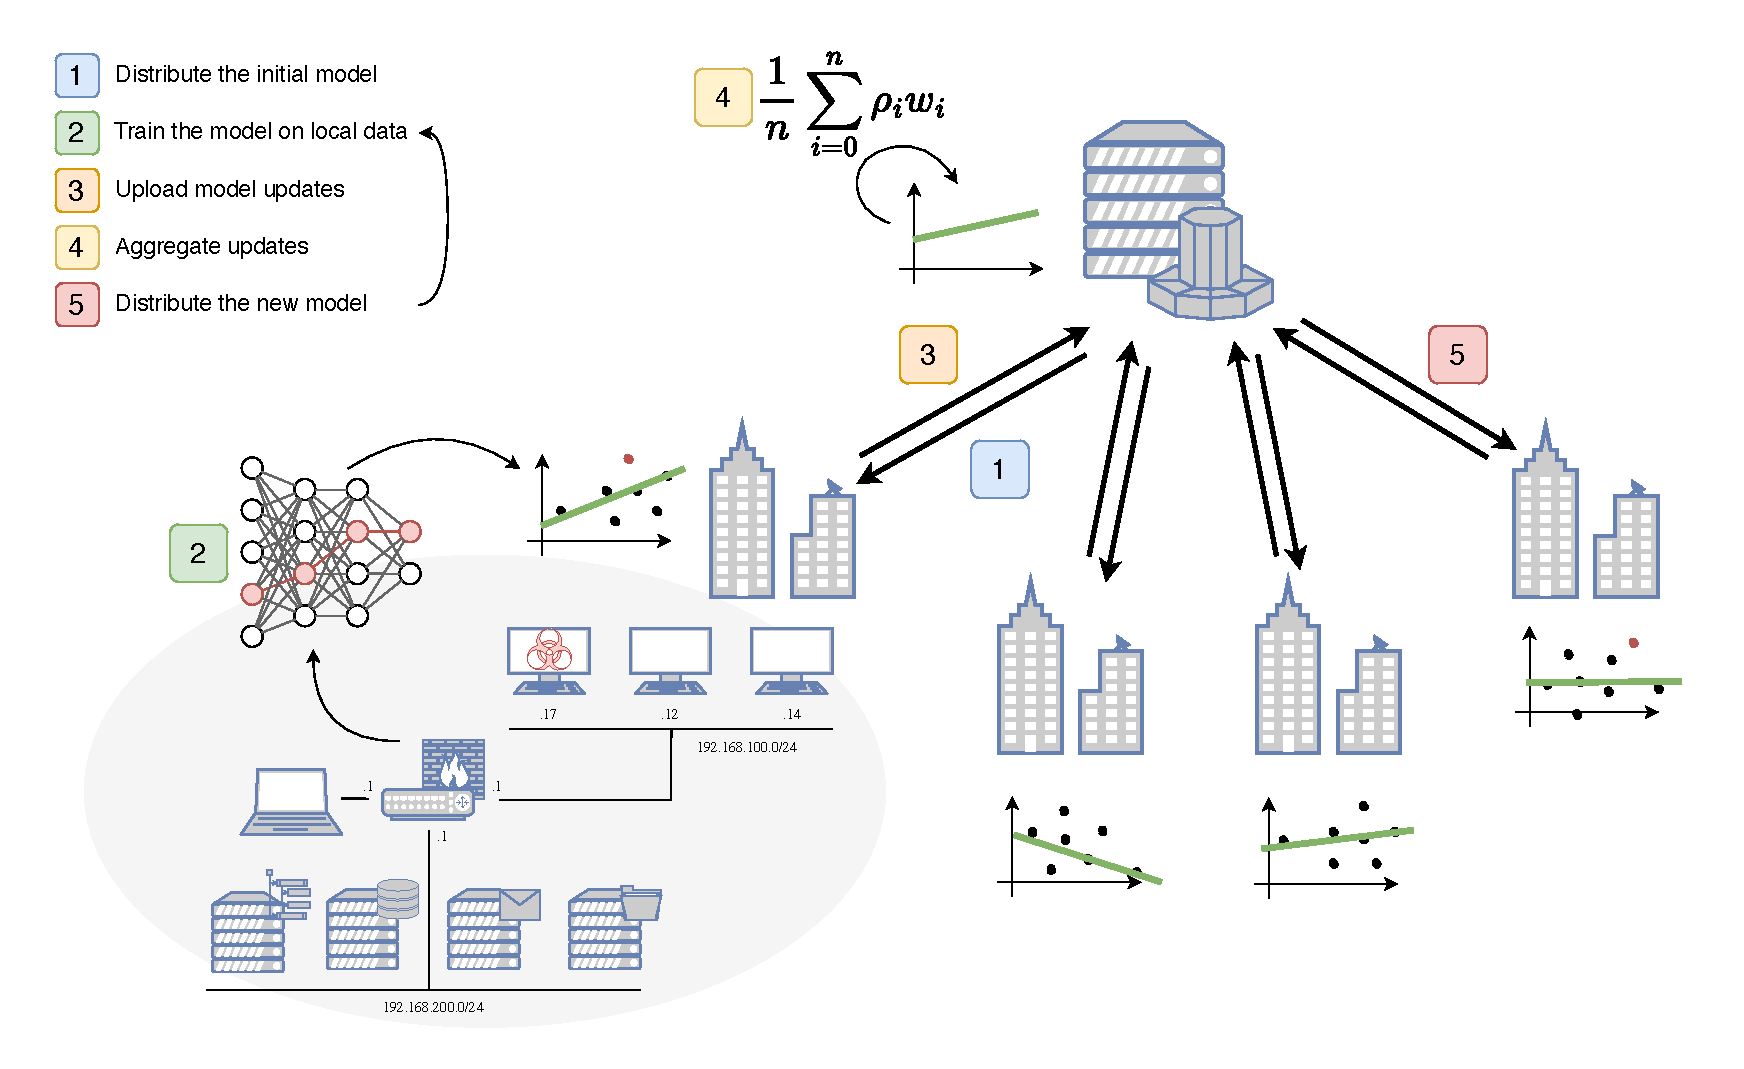
\includegraphics[width=\linewidth]{figures/intro/fl.drawio.pdf}
      \end{figure}
    \end{column}
  \end{columns}

  \fcitefootnote{mcmahan_Communicationefficientlearningdeep_2017}
\end{frame}


\begin{frame}{Case Study}
  \textbf{Collaborative Intrusion Detection between Distributed Organizations}
  \begin{itemize}
    \item Each organization has its own NIDS and monitors an information system via its network traffic.
    \item They want to improve their detection capabilities.
    \item Share knowledge about new attacks or specific devices.
  \end{itemize}
  
  \pause
  \textbf{Byzantine contributions}
  \begin{itemize}
    \item No guarantees on the quality of the contributions.
    \item Can be intentional, due to poor data quality, or due to data distribution mismatches.
  \end{itemize}
\end{frame}

\begin{frame}{Case Study -- Generalization}
  \textbf{A cross-silo use case}~\cite{kairouz_AdvancesOpenProblems_2021}:
  \begin{itemize}
    \item few clients (\ie, 10--100);
    \item consequent amount of data, high heterogeneity;
    \item high availability, significant computing resources.
  \end{itemize}
\end{frame}

\begin{frame}{Heterogeneity Headaches}
  
  \begin{columns}
    \begin{column}{.5\textwidth}
      \includegraphics<1>[width=\linewidth]{figures/intro/heterogeneity/introducing_heterogeneity.pdf}
      \includegraphics<2>[width=\linewidth]{figures/intro/heterogeneity/introducing_heterogeneity_aggregated.pdf}
      \includegraphics<3>[width=\linewidth]{figures/intro/heterogeneity/introducing_poisoning.pdf}

    \end{column}

    \begin{column}{.5\textwidth}

      \textcolor<3->{lightgray}{%
      \textbf{Challenge I}: \textit{Too much heterogeneity leads to poor performance\dots}
      }
      \only<1-2>{%
        \begin{itemize} \small
          \item How to handle different feature sets, data distributions?
          \item How to consider models that are dissimilar yet "contain" relevant knowledge?
        \end{itemize}
      }
      \vspace{1ex}


      \textcolor<1-2>{lightgray}{%
      \textbf{Challenge II}: \textit{Difficult to identify malicious contributions when models are different\dots}
      }
      
      \only<3>{%
        \begin{itemize} \small
          \item Are model "dissimilar" because they are different, or because they are malicious/poisoned?
        \end{itemize}
      }
      \vspace{1ex}
      
    \end{column}
  \end{columns}  
\end{frame}

\begin{frame}{Problem Statement}
  \begin{block}{Quality Assessment in Heterogeneous Settings}
    For $n$ participants $p_i$ and their local datasets $d_i$ of unknown similarity, each participant uploads a model update $w_i^r$ at each round $r$. Given $P = \{ p_1, p_2, \dots, p_n \} $ and $W = \{ w_1^r, w_2^r, \dots, w_n^r \} $, how can one assess the quality of each participant’s contribution without making assumptions on the data distribution across the datasets $d_i$?
  \end{block}
\end{frame}

\begin{frame}{Outline}
  \centering
  \begin{minipage}[t]{.8\textwidth}
    \tableofcontents%[hideallsubsections,]
  \end{minipage}
\end{frame}

